\documentclass[border=8pt,tikz]{standalone}
\usepackage{amsmath,amssymb}
\usepackage{tikz}
\usetikzlibrary{arrows.meta,calc,decorations.pathreplacing,decorations.pathmorphing,patterns,shapes.geometric,positioning,shadings}

\begin{document}
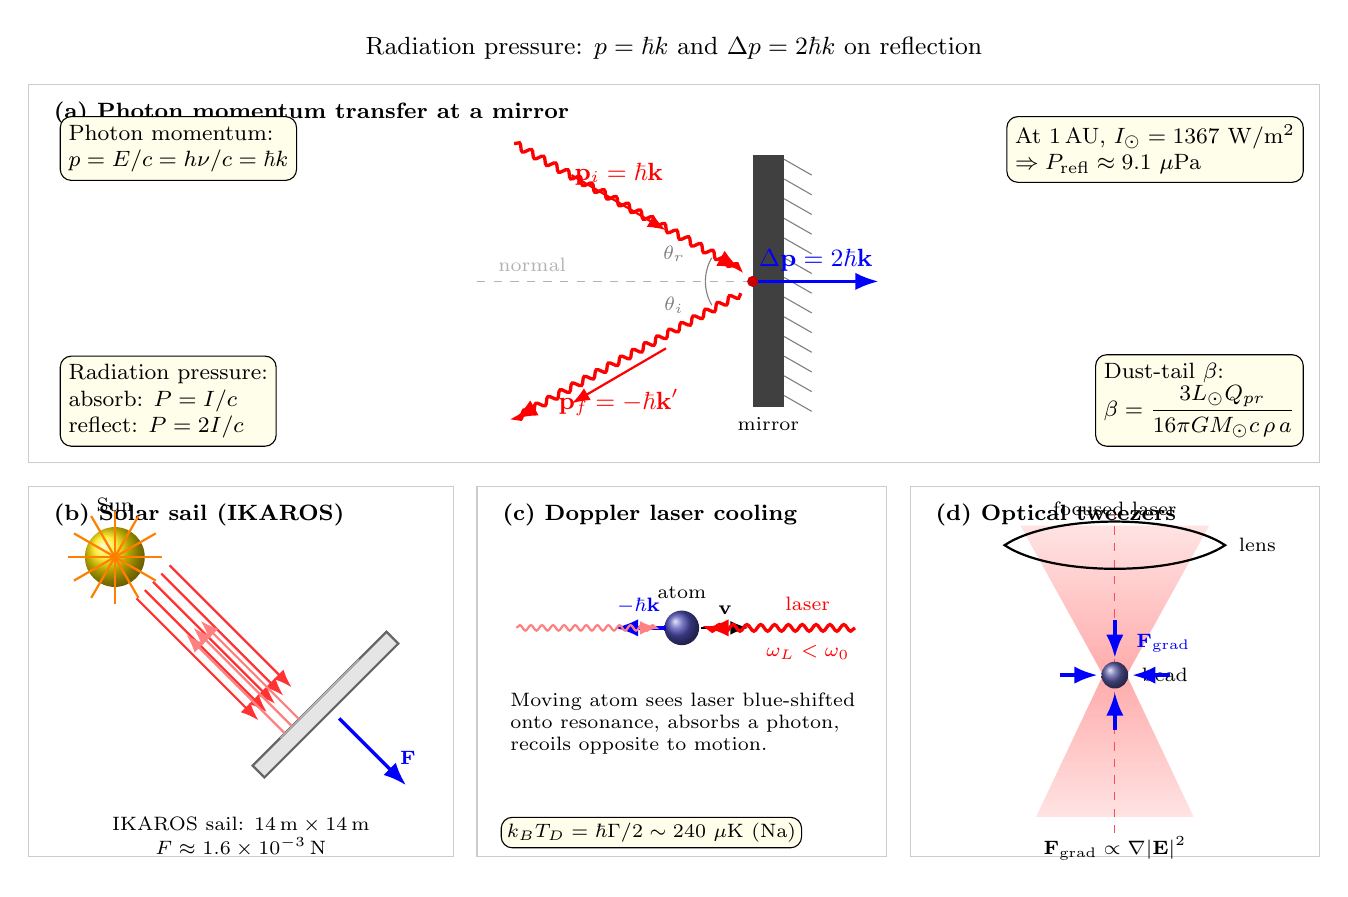
\begin{tikzpicture}[>=Latex,font=\small]

% ================================================================
% Top title
% ================================================================
\node[anchor=south,font=\small] at (8.0,9.3)
  {Radiation pressure: $p=\hbar k$ and $\Delta p = 2\hbar k$ on reflection};

% ================================================================
% Layout:  MAIN figure (top) spanning full width  y in [4.5, 9.0]
%          Three sub-panels (b,c,d) in bottom row  y in [-0.5, 4.0]
% ================================================================

% ----------------------------------------------------------------
% (a) MAIN FIGURE: photon reflecting off a mirror
% Box: x in [0, 16], y in [4.5, 9.0]
% ----------------------------------------------------------------
\begin{scope}
  % Outer frame
  \draw[gray!40,thin] (-0.2,4.3) rectangle (16.2,9.1);
  \node[anchor=north west,font=\footnotesize\bfseries] at (0.0,9.0) {(a) Photon momentum transfer at a mirror};

  % Mirror: dark grey filled rectangle, vertical at x = 9.0
  \fill[black!75] (9.0,5.0) rectangle (9.4,8.2);
  % Hatching on back side of mirror
  \foreach \yy in {5.15,5.4,5.65,5.9,6.15,6.4,6.65,6.9,7.15,7.4,7.65,7.9,8.15}{
    \draw[black!50,thin] (9.4,\yy) -- (9.75,\yy-0.2);
  }
  \node[font=\scriptsize,anchor=north] at (9.2,5.0) {mirror};

  % Mirror normal (dashed horizontal line from mirror to the left, for reference)
  \draw[gray!60,dashed,thin] (5.5,6.6) -- (9.0,6.6);
  \node[gray!60,font=\scriptsize,anchor=south] at (6.2,6.6) {normal};

  % Incoming photon: red wavy line with arrow, going down-right to strike mirror at (9.0,6.6) from upper-left
  \draw[red,very thick,decorate,decoration={snake,amplitude=1.2pt,segment length=5pt},->]
      (5.97,8.35) -- (8.85,6.75);

  % Reflected photon: red wavy with arrow, going down-left
  \draw[red,very thick,decorate,decoration={snake,amplitude=1.2pt,segment length=5pt},->]
      (8.85,6.45) -- (5.97,4.85);

  % Momentum vector of incoming photon
  \draw[red,thick,->] (6.7,7.95) -- (7.9,7.25);
  \node[red,font=\small,anchor=south] at (7.3,7.7) {$\mathbf{p}_i=\hbar \mathbf{k}$};

  % Momentum vector of reflected photon
  \draw[red,thick,->] (7.9,5.75) -- (6.7,5.05);
  \node[red,font=\small,anchor=north] at (7.3,5.35) {$\mathbf{p}_f = -\hbar \mathbf{k}'$};

  % Change of momentum transferred to the mirror
  \draw[blue,very thick,->] (9.0,6.6) -- (10.6,6.6);
  \node[blue,font=\small,anchor=south] at (9.8,6.6) {$\Delta \mathbf{p} = 2\hbar \mathbf{k}$};

  % Angle arcs
  \draw[gray,thin] (8.4,6.6) arc (180:210:0.6);
  \node[gray,font=\scriptsize] at (8.0,6.3) {$\theta_i$};
  \draw[gray,thin] (8.4,6.6) arc (180:150:0.6);
  \node[gray,font=\scriptsize] at (8.0,6.95) {$\theta_r$};

  % Photon particle dot at strike
  \fill[red!80!black] (9.0,6.6) circle (2pt);

  % Formula boxes
  \node[draw,rounded corners,fill=yellow!8,inner sep=3pt,font=\footnotesize,align=left,anchor=north west]
    at (0.2,8.7)
    {Photon momentum:\\ $p = E/c = h\nu/c = \hbar k$};

  \node[draw,rounded corners,fill=yellow!8,inner sep=3pt,font=\footnotesize,align=left,anchor=south west]
    at (0.2,4.5)
    {Radiation pressure:\\ absorb: $P=I/c$ \\ reflect: $P=2I/c$};

  \node[draw,rounded corners,fill=yellow!8,inner sep=3pt,font=\footnotesize,align=left,anchor=north east]
    at (16.0,8.7)
    {At $1\,\mathrm{AU}$, $I_\odot=1367~\mathrm{W/m^2}$ \\
     $\Rightarrow P_{\text{refl}} \approx 9.1~\mathrm{\mu Pa}$};

  \node[draw,rounded corners,fill=yellow!8,inner sep=3pt,font=\footnotesize,align=left,anchor=south east]
    at (16.0,4.5)
    {Dust-tail $\beta$:\\ $\beta = \dfrac{3 L_\odot Q_{pr}}{16\pi G M_\odot c\, \rho\, a}$};
\end{scope}

% ================================================================
% Sub-panels (b), (c), (d)
% ================================================================

% ---------------- (b) Solar sail ----------------
\begin{scope}[shift={(0.0,0.0)}]
  \draw[gray!40,thin] (-0.2,-0.7) rectangle (5.2,4.0);
  \node[anchor=north west,font=\footnotesize\bfseries] at (0.0,3.9) {(b) Solar sail (IKAROS)};

  % Sun: yellow disk with rays
  \shade[ball color=yellow!80!orange] (0.9,3.1) circle (0.38);
  \foreach \ang in {0,30,60,90,120,150,180,210,240,270,300,330}{
     \draw[orange,thick] (0.9,3.1) -- +(\ang:0.6);
  }
  \node[font=\scriptsize,anchor=south] at (0.9,3.55) {Sun};

  % Light rays (parallel red arrows) from sun toward the sail
  \foreach \off in {-0.5,-0.2,0.1,0.4,0.7}{
     \draw[red!80,thick,->,shorten >=2pt]
       ($(1.35,2.75)+(\off*0.35,\off*0.35)$) -- ($(2.95,1.15)+(\off*0.35,\off*0.35)$);
  }

  % Reflective sail: tilted square (parallelogram)
  \fill[gray!20,draw=black!60,thick]
      (3.5-0.85, 1.3-0.85) -- (3.5+0.85, 1.3+0.85)
      -- (3.5+0.85+0.15, 1.3+0.85-0.15) -- (3.5-0.85+0.15, 1.3-0.85-0.15) -- cycle;
  % Sail grid diagonals
  \draw[gray!55,thin] (3.5-0.5,1.3-0.5) -- (3.5+0.5,1.3+0.5);
  \draw[gray!55,thin] (3.5-0.25,1.3-0.25) -- (3.5+0.25,1.3+0.25);

  % Reflected rays from sail (going back toward upper-left)
  \foreach \off in {-0.3,0.0,0.3}{
     \draw[red!50,thick,->,shorten >=2pt]
       ($(3.15,0.95)+(\off*0.3, \off*0.3)$) -- ($(1.85,2.25)+(\off*0.3, \off*0.3)$);
  }

  % Thrust arrow
  \draw[blue,very thick,->] (3.75,1.05) -- (4.6,0.2);
  \node[blue,font=\scriptsize,anchor=west] at (4.4,0.55) {$\mathbf{F}$};

  % Labels
  \node[font=\scriptsize,align=center] at (2.5,-0.30) {IKAROS sail: $14\,\text{m}\times 14\,\text{m}$};
  \node[font=\scriptsize,align=center] at (2.5,-0.58) {$F\approx 1.6\times 10^{-3}\,\mathrm{N}$};
\end{scope}

% ---------------- (c) Doppler laser cooling ----------------
\begin{scope}[shift={(5.7,0.0)}]
  \draw[gray!40,thin] (-0.2,-0.7) rectangle (5.0,4.0);
  \node[anchor=north west,font=\footnotesize\bfseries] at (0.0,3.9) {(c) Doppler laser cooling};

  % Atom: blue-grey small circle
  \shade[ball color=blue!40!gray] (2.4,2.2) circle (0.22);
  \node[font=\scriptsize,anchor=south] at (2.4,2.45) {atom};

  % Atom velocity arrow
  \draw[black,thick,->] (2.65,2.2) -- (3.25,2.2);
  \node[font=\scriptsize,anchor=south] at (2.95,2.25) {$\mathbf{v}$};

  % Counter-propagating red laser from the right
  \draw[red,very thick,decorate,decoration={snake,amplitude=1.2pt,segment length=5pt},->]
      (4.6,2.2) -- (2.7,2.2);
  \node[red,font=\scriptsize,anchor=south] at (4.0,2.3) {laser};
  \node[red,font=\scriptsize,anchor=north] at (4.0,2.1) {$\omega_L < \omega_0$};

  % Recoil arrow on atom: push-back (blue) to the left
  \draw[blue,very thick,->] (2.2,2.2) -- (1.55,2.2);
  \node[blue,font=\scriptsize,anchor=south] at (1.85,2.25) {$-\hbar \mathbf{k}$};

  % Co-propagating laser from the left (symmetric)
  \draw[red!50,thick,decorate,decoration={snake,amplitude=1pt,segment length=4pt},->]
      (0.3,2.2) -- (2.1,2.2);

  % Caption lines
  \node[font=\scriptsize,align=left,anchor=north west] at (0.1,1.5)
    {Moving atom sees laser blue-shifted\\
     onto resonance, absorbs a photon,\\
     recoils opposite to motion.};
  \node[draw,rounded corners,fill=yellow!8,inner sep=2pt,font=\scriptsize,anchor=south west]
    at (0.1,-0.6) {$k_B T_D = \hbar\Gamma/2 \sim 240~\mathrm{\mu K}$ (Na)};
\end{scope}

% ---------------- (d) Optical tweezers ----------------
\begin{scope}[shift={(11.2,0.0)}]
  \draw[gray!40,thin] (-0.2,-0.7) rectangle (5.0,4.0);
  \node[anchor=north west,font=\footnotesize\bfseries] at (0.0,3.9) {(d) Optical tweezers};

  % Focusing Gaussian beam (cone above waist, expanding below)
  \shade[top color=red!20,bottom color=red!60,opacity=0.55]
     (1.2,3.5) -- (3.6,3.5) -- (2.55,1.6) -- (2.25,1.6) -- cycle;
  \shade[top color=red!60,bottom color=red!20,opacity=0.55]
     (2.25,1.6) -- (2.55,1.6) -- (3.4,-0.2) -- (1.4,-0.2) -- cycle;

  % Beam axis
  \draw[red!70,dashed,thin] (2.4,3.7) -- (2.4,-0.4);

  % Lens symbol at top (biconvex)
  \draw[thick] (1.0,3.25) .. controls (1.6,3.65) and (3.2,3.65) .. (3.8,3.25)
              .. controls (3.2,2.85) and (1.6,2.85) .. (1.0,3.25) -- cycle;
  \node[font=\scriptsize,anchor=west] at (3.85,3.25) {lens};

  % Particle at beam waist
  \shade[ball color=blue!30!gray] (2.4,1.6) circle (0.17);
  \node[font=\scriptsize,anchor=west] at (2.62,1.6) {bead};

  % Gradient force arrows pointing toward focus
  \draw[blue,very thick,->] (1.7,1.6) -- (2.18,1.6);
  \draw[blue,very thick,->] (3.1,1.6) -- (2.62,1.6);
  \draw[blue,very thick,->] (2.4,2.3) -- (2.4,1.82);
  \draw[blue,very thick,->] (2.4,0.9) -- (2.4,1.38);
  \node[blue,font=\scriptsize,anchor=north west] at (2.55,2.25) {$\mathbf{F}_\text{grad}$};

  % Labels
  \node[font=\scriptsize,anchor=south] at (2.4,3.5) {focused laser};
  \node[font=\scriptsize,align=center] at (2.4,-0.60) {$\mathbf{F}_\text{grad}\propto \nabla|\mathbf{E}|^2$};
\end{scope}

\end{tikzpicture}
\end{document}
